% Chapter 4

\chapter{LRR-CED: Low-Resolution Reconstruction aware Convolutional Encoder-Decoder Network  for Direct Sparse-View CT Image Reconstruction} % Main chapter title
\chaptermark{LRRCED}
\label{Chapter5} % For referencing the chapter elsewhere, use \ref{Chapter1} 

Sparse-view \ac{CT} reconstruction has been at the forefront of research in medical imaging. Reducing the total X-ray radiation dose to the patient while preserving the reconstruction accuracy is a big challenge. The sparse-view approach is based on reducing the number of rotation angles, which leads to poor quality reconstructed images as it introduces several artifacts. These artifacts are more clearly visible in traditional reconstruction methods like the \ac{FBP} algorithm. Over the years, several model-based iterative and more recently deep learning-based methods have been proposed to improve sparse-view \ac{CT} reconstruction. Many deep learning-based methods improve \ac{FBP}-reconstructed images as a post-processing step. In this work, we propose a direct deep learning-based reconstruction that exploits the information from low-dimensional \ac{FBP} estimates, to learn the  projection-to-image mapping. This is done by concatenating the \ac{FBP} estimate at multiple resolutions in the decoder part of a \ac{CED}. This approach is investigated on two different networks, based on Dense Blocks and U-Net to show that a direct mapping can be learned from a sinogram to an image.  The results are compared to a post-processing deep learning method and an iterative method that uses a \ac{TV} regularization. 


\section{Main Contribution}

The main drawbacks of current deep learning-based direct image reconstruction algorithms are the tedious training process necessary to train large networks with large number of trainable parameters and the requirement of high memory in case of high-resolution \ac{CT} images. 
In this work we propose a new method for direct deep learning based sparse-view \ac{CT} image reconstruction with fully convolutional networks. We use two networks, namely Fully Convolutional Densenets \cite{jegou2017one} and U-Net \cite{ronneberger2015u}. An important characteristic of both these architectures \cite{jegou2017one,ronneberger2015u} is the presence of concatenation from the encoding layers to the decoding layers that ensures the usage of features from the input for the reconstruction. Specifically, for application in sparse-\ac{CT} image reconstruction, the network would have sparse-view sinograms as input and reconstructed images as output. The original application in the medical imaging field of both these architectures was in image segmentation, where the image-to-image mapping operates in the same image domain. Medical image reconstruction on the other hand involves mapping between two different domains (sinogram to image). In order to help the network to learn the mapping from sinogram to image, we propose the use of \ac{FBP} image estimates of the sparse sinograms and concatenate them with the feature maps of the decoder. 

% \AP{Here the motivation for this "intuition" should be stated maybe you can introduce some simple notation already here: Given that we only have access to sparse measurement data (sinogram $\boldy$), we can enforce that the inverse mapping $f$ at each layer/ sub-resolution of the network is consistent in the measurement domain. That is 	$\boldL f(\boldy) = \boldy$.  this can be achieved by using concatenating as feature maps a (fast) low-resolution FBP for each or a subset of levels of the network. While this leads to a massive reduction of the parameters (number of layers) required in the network, the network parameters has to be trained accordingly since the above mentioned constraint is not enough to learn the inverse mapping, as it cannot capture information about the image $\boldx$ outside the range of the physical under-determined operator $\boldL$ (Radon transform for CT). Do not put details of the implementation in the introduction rather put the general idea behind.}

Given that we only have access to sparse measurement data, taking the form of a sinogram $\boldy$, we can enforce that the inverse mapping $\boldf$ at each layer/sub-resolution of the network is consistent in the measurement domain. That is $\boldP \boldf(\boldy) = \boldy$. This can be achieved by concatenating, as feature maps, (fast) low-resolution \ac{FBP}-reconstructed images for each or a subset of the network levels. While this leads to a massive reduction of the parameters (fully convolutional layers instead of fully-connected) required in the network, the above-mentioned constraint is not enough to learn the inverse mapping as it cannot capture information about the image $\boldx$ outside the range of the physical under-determined operator $\boldP$ (Radon transform for CT). Hence, the network needs to be trained accordingly.

Once the network is trained, these custom concatenations enable architectures that were previously used for denoising/artifact removal to learn a mapping from sparse sinograms to full-resolution \ac{CT} images. One characteristic feature of reconstructions generated by deep learning-based methods is the blurriness of the outputs. To counteract this we used perceptual loss involving features extracted from two different levels of $\mathrm{VGG16}$ network (Block 1 and Block 3). Since the exclusive use of perceptual loss results in unrealistic artifacts we couple it with a $L_1$ loss. A general representation of the proposed approach is depicted in Figure~\ref{fig:ge}. It consists of a \ac{CED} network with two blocks in both the encoder and the decoder that takes in as input a reshaped sparse sinogram which has the same dimensions as the output image. A concatenation of two resolutions $h_1 \times w_1$ and $h_2 \times w_2$ is incorporated in the decoder. 

The main contributions of our work are summarized as follows:
\begin{itemize}
	\item A new approach for sparse-view \ac{CT} image reconstruction using fully-convolutional networks
	\item Use of lower resolution \ac{FBP} estimates which enable the networks that are predominantly used for denoising to learn the more complex mapping from sinogram to image domain. 
	\item Two neural networks are implemented to test this approach using different levels of sparsity in the sinograms. 
\end{itemize}

\begin{figure}[!htbp]
	\centering
	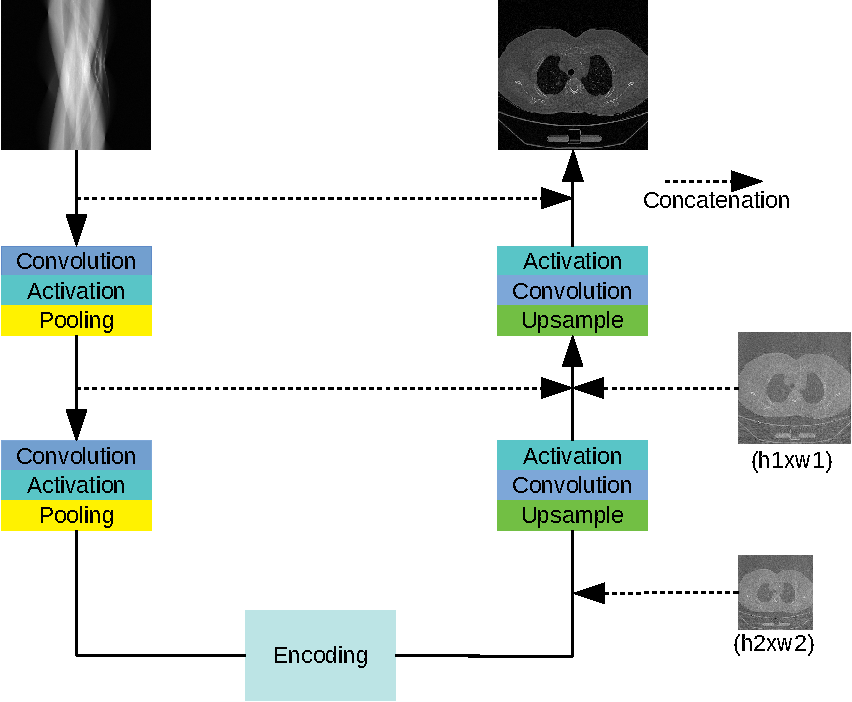
\includegraphics[width=0.7\linewidth]{general_enc-crop.pdf}
	\caption{General representation of an encoder-decoder architecture with fully convolutional layers and the proposed \ac{FBP} concatenations ($\boldx_1$ and $\boldx_2$) at two different resolutions $h_1 \times w_1$ and $h_2 \times w_2$}
	\label{fig:ge}
\end{figure}


\section{Methods}

\subsection{Proposed Low Resolution Reconstruction aware \ac{CED} Model}

Supervised deep learning-based methods learn the mapping between the measurement $\boldy$ and the corresponding reconstructed image $\boldx$. In the case of direct deep learning-based image reconstruction this mapping is typically learned via neural networks which can be represented as a function $\boldf_{\Theta}\colon \bbR^n \to \bbR^m$ with trainable parameters $\Theta$: 
\begin{equation}\label{eq:dl}
\boldxhat = \boldf_{\Theta}(\boldy) \, .
\end{equation}  
where, $\boldxhat$ is the predicted image. 

Most of the works in direct reconstruction for sparse-view \ac{CT} represent $\boldf$ with a neural network with fully-connected layers. These networks require huge memory and large datasets for training. As an alternative to this, we propose the use of fully convolutional encoder-decoder networks that have lesser trainable parameters and are faster to train. 
The main idea is to enforce data consistency by providing estimates at different resolutions $\boldxhat_r$, $r = 1, \ldots, R$:
\begin{equation}\label{eq:d}
\boldxhat = \boldf_{\Theta}(\boldy,   (\boldxhat_r)_{r=1}^R    ) 
\end{equation}  
where each $\boldxhat_r \in \bbR^{m_r}$, $m_r < m$, is an approximate solution of
\begin{equation}\label{eq:xr}
\boldy = \boldP \boldU_r \boldxhat_r
\end{equation} 
with $\boldU_r\in\bbR^{m\times m_r}$ being an upsampling operator.

In a typical \ac{CED}, the encoder learns the representation of the input domain and the decoder learns to map this representation to the corresponding image in the output domain. In the specific case of a \ac{CED} for medical image reconstruction, the encoder operates in the sinogram space and the decoder in the image space. Based on this hypothesis, we propose to concatenate the estimates at different levels of the decoder part of the network. The function of these concatenations is to help the network learn the structure of the image. The feature maps at different levels of the decoder have different resolutions. Hence, concatenating the estimate $\boldxhat_r$ at different levels requires the estimate to be of the appropriate resolution. The different convolutional layers in the decoder work towards arriving at a clear reconstructed image that is free of artifacts and noise. The estimate $\boldxhat_r$ is obtained with a sparse sinogram, hence it is artifact-ridden and noisy. Therefore, concatenating the estimate $\boldxhat_r$ at a level closer to the output resolution is counter productive as the network has lesser number of convolutional layers to correct the noise and artifacts. On the other hand the estimate at lower resolutions has lesser structural information compared to the estimates at higher resolution. The selection of $\boldxhat_r$ should ensure a balance between aiding the network to learn the structure of the image and enabling it to correct the artifacts and noise. 

Our method, namely \ac{LRRCED}, was implemented with $R=2$ and the image estimates $\boldxhat_r$ were obtained by \ac{FBP} at lower resolution. With the help of a series of experiments, we determined the best possible configuration for concatenating $\boldxhat_r$. In section Section~\ref{sec:concat}, we present quantitative evaluation of the effect of these concatenations on the reconstructed images. 

We investigate \ac{LRRCED} with two different variations for $\boldf$, \ac{LRRCED}(D) with Fully Convolutional DenseNets and \ac{LRRCED}(U) with U-Net, which are discussed in Section~\ref{sec:FCDN} and Section~\ref{sec:UNet}. 




\subsubsection{Fully Convolutional Dense Networks}\label{sec:FCDN}

A fully convolutional dense network was used as first variation of \ac{LRRCED}. Dense networks \cite{huang2017densely} are based on the hypothesis that connecting all the layers to each other in a feed forward fashion leads to higher accuracy and easier training of the network. A typical dense block of three layers is depicted in Figure~\ref{fig:db}. The extension of dense networks for image segmentation was proposed by \cite{jegou2017one}. The three  blocks involved in the construction of this network are \ac{DB} with $l$ number of layers, \ac{TU} and \ac{TD}. The combination of these three blocks helps in building an encoder-decoder structure suitable for tasks dealing with image-to-image domain transfer. Each layer consists of batch normalization, \ac{ReLU} activation and $3\times 3$ convolution. \ac{TD} includes: batch normalization, \ac{ReLU}, $1\times 1$ Convolution and $2\times 2$ max pooling. Finally, \ac{TU}  includes a $3\times 3$ transposed convolution with stride $2$. The important modification to the architecture blocks in our work is the removal of the dropout layers. The fully convolutional dense network with proposed concatenations is represented in Figure~\ref{fig:dn}. For the sake of representation we included only $5$ dense blocks in the figure. The complete architecture details are given in Table~\ref{table:1a}. 


\subsubsection{U-Net}\label{sec:UNet}

One of the most established architectures for image-to-image translation is U-Net \cite{ronneberger2015u}, which we used as second variation of \ac{LRRCED} (called from here on-wards as \ac{LRRCED}(U)).
 
A typical U-Net consists of Convolution, Activation (\ac{ReLU}) and Pooling layers in the encoder and Upsampling, Convolution and Activation in the decoder. We have used U-Net without the dropout, similar to the dense network. The U-Net is represented in Figure~\ref{fig:un}. 

\begin{figure}[!htbp]
	\begin{subfigure}{.25\textwidth}
		\centering
		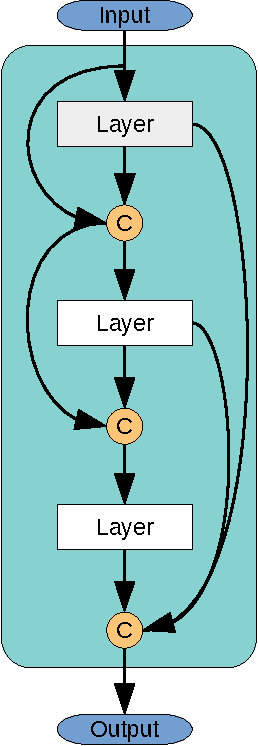
\includegraphics[width=0.4\linewidth]{dense_block-crop.pdf}
		\caption{Dense Block}
		\label{fig:db}
	\end{subfigure}%
	\begin{subfigure}{.40\textwidth}
		\centering
		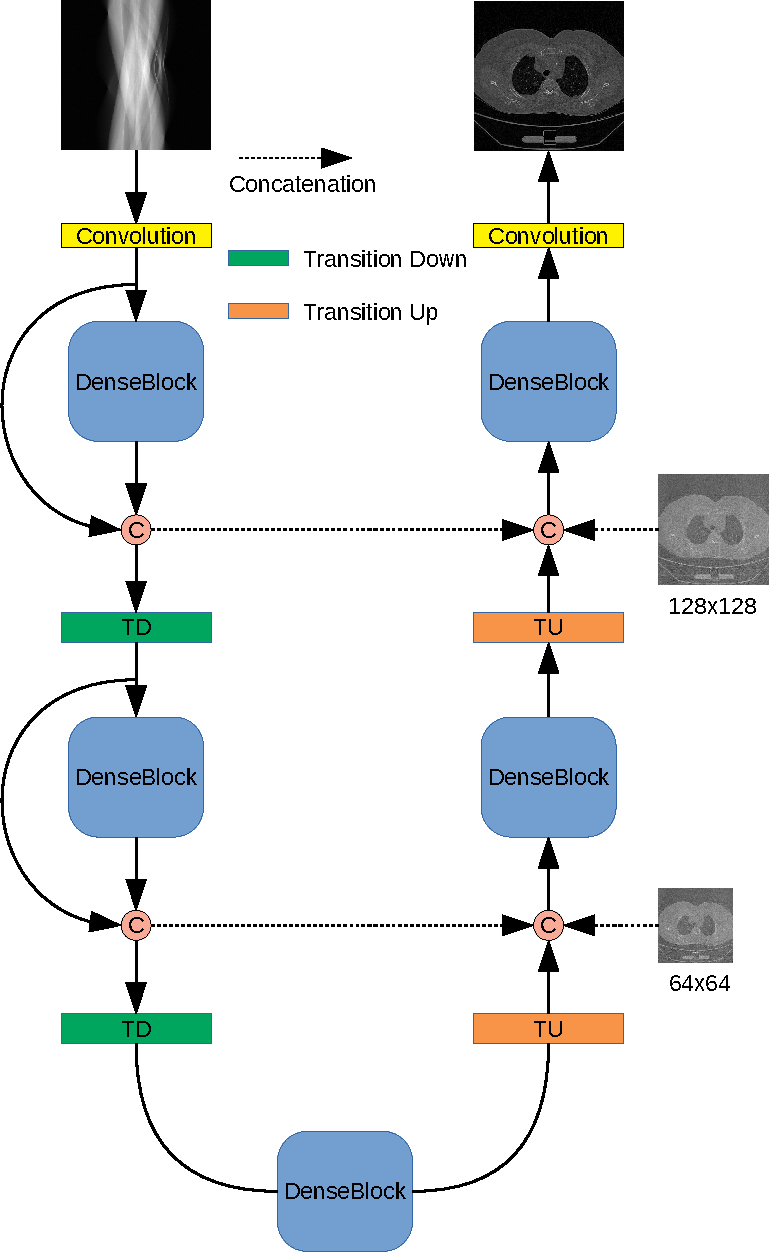
\includegraphics[width=1.0\linewidth]{dense_net-crop.pdf}
		\caption{\ac{LRRCED}(D)}
		\label{fig:dn1}
	\end{subfigure}%
	\begin{subfigure}{.35\textwidth}
		\centering
		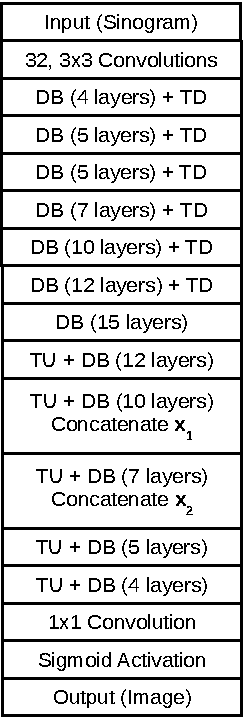
\includegraphics[width=0.5\linewidth]{arc-crop.pdf}
		\caption{Architecture Summary}
		\label{fig:dn2}
	\end{subfigure}%
	\caption{Different components of \ac{LRRCED}(D): \subref{fig:db} Representation of a dense block with three layers. \subref{fig:dn1} \ac{LRRCED}(D): Fully convolutional dense network with $\boldx_1$ at $64\times64$ and $\boldx_2$ at $128\times128$. \subref{fig:dn2} Complete architecture summary}
	\label{fig:den}
\end{figure}


\begin{figure}[!htbp]
	\begin{subfigure}{.60\textwidth}
		\centering
		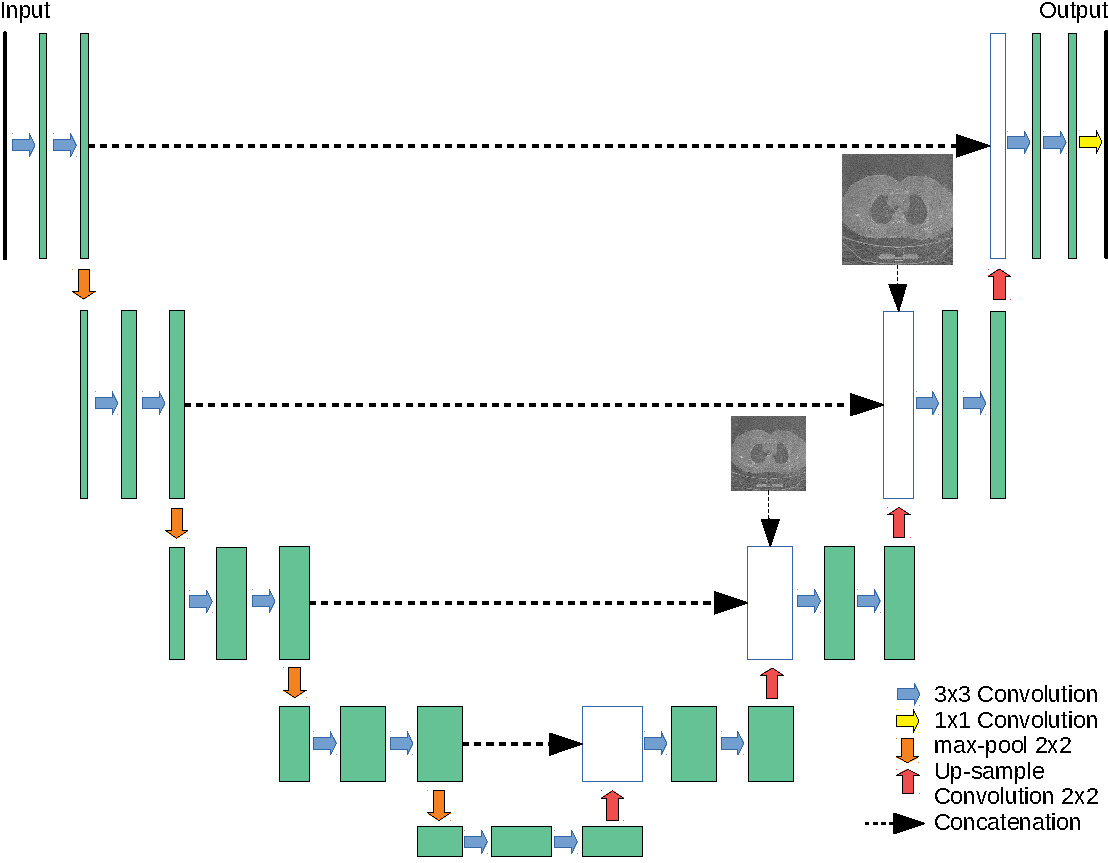
\includegraphics[width=1.0\linewidth]{u_net-crop.pdf}
		\caption{\ac{LRRCED}(U)}
		\label{fig:un}
	\end{subfigure}%
	\begin{subfigure}{.40\textwidth}
		\centering
		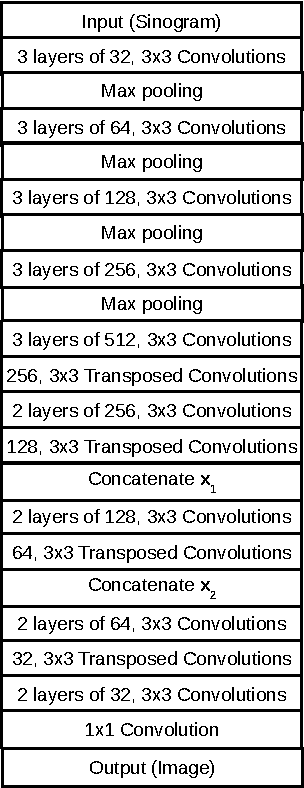
\includegraphics[width=0.7\linewidth]{unet_details-crop.pdf}
		\caption{Architecture Summary}
		\label{fig:ud}
	\end{subfigure}%
	\caption{Different components of \ac{LRRCED}(U): \subref{fig:un} \ac{LRRCED}(U): U-Net with $\boldx_1$ at $64\times64$ and $\boldx_2$ at $128\times128$. \subref{fig:ud} Complete architecture summary.}
	\label{fig:unet}
	
\end{figure}

\subsubsection{Loss Function}
The aim of a supervised data-driven image reconstruction task is to predict an image that is as close as possible to the \ac{GT} image. The appropriate loss function to achieve this is the \ac{MAE} which is defined as follows:
\begin{equation}
\mathrm{MAE}(\boldx^\star, \boldxhat) = \frac{1}{m}   \sum_{j=1}^m |x^\star_j - \hat{x}_j|
\end{equation}
where $\boldx^\star =  [x_1^\star, \dots , x_m^\star]^\top \in \mathbb{R}^m$ and $\boldxhat= [\hat{x}_1, \dots , \hat{x}_m]^\top \in \mathbb{R}^m$ are respectively the true image and predicted image.

In order to improve the resolution of reconstructed images, many deep learning approaches have used the perceptual loss as proposed by \cite{johnson2016perceptual}. This loss uses a pre-trained neural network to extract features from the predicted image and the \ac{GT}. It can be defined as follows:

\begin{equation}
P_k(\boldx^\star,\boldxhat) =  |[\mathrm{VGG16}]_k(\boldx^\star) - [\mathrm{VGG16}]_k( \boldxhat)|, \quad k =1,\dots,5 \,  
\end{equation}
where $[\mathrm{VGG16}]_k(\boldx^\star)$ and $[\mathrm{VGG16}]_k( \boldxhat)$ are the features extracted from block $k$ of the $\mathrm{VGG16}$ neural network \cite{simonyan2014very} with respectively the \ac{GT} and the predicted image as inputs. The features extracted from higher layers of the neural network contain generic information (edges, contrast, etc.) while the deeper layers have finer task-specific details. The VGG16 network was pre-trained on Image-Net data \cite{deng2009imagenet} which is far from a medical context. Hence, the higher-level generic features were found to be more relevant for the task of medical image reconstruction. We observed that using extracted features from two different levels, namely Block 1 and Block 3, of the VGG16 network proved to be most effective. 

The final loss function that was used for training both the aforementioned networks is defined as follows: 
\begin{equation}\label{eq:loss}
\mathcal{L}(\boldx^\star,\boldxhat) = \alpha\mathrm{MAE}(\boldx^\star, \boldxhat)+\beta(P_{1}(\boldx^\star,\boldxhat)+P_{3}(\boldx^\star,\boldxhat))
\end{equation}
where $P_{1}$ and $P_{3}$ are perceptual loss from the extracted features of the two different blocks above-mentioned, $\alpha$ and $\beta$ are weights which were set to $10$ and $0.5$ during the training phase.  


\section{Dataset}
The data used in this work is from the \ac{Lung} \cite{Lung20,clark2013cancer}. Details of the dataset are given in Table~\ref{table:2a}. The images in this dataset were reconstructed using \ac{FBP} on full-angular coverage measurement data. We used the ASTRA toolbox \cite{van2016fast}, for data processing to create the projection-image pairs.  A fan-beam geometry with a source to detector distance at $1500$ mm and source to the center of the rotation at $1000$ mm were considered. The number of detectors was set to $700$ and the number of angles was varied to generate different levels of sparsity ($N_\mathrm{a}=60,90$ and $120$). The noise-free projection data were obtained using the Beer-Lambert law \eqref{eq:CT} with an input emission intensity of $10^5$. The final projection data were obtained by adding Poisson noise (i.e., \eqref{eq:poisson}) to the noise-free projection data. We finally generated the \ac{FBP} estimates from the noise-added sparse-projections which were used in training the networks as explained previously. Sample images from the dataset are shown in Figure~\ref{fig:data}. 



\begin{table}[ht!]
	\caption{Dataset Description}
	\label{table:1}
	\centering
	\begin{tabular}{||c|c||} 
		\hline
		Dataset Statistics &  \\ [0.5ex] 
		\hline
		Modalities & CT   \\ 
		\hline
		Number of Participants  & 355  \\
		\hline
		Number of Studies  & 436  \\
		\hline
		Number of Series & 1295 \\ 
		\hline
		Number of 2-D Image slices & 251,135 \\ 
		\hline
		CT Matrix size & 512 \\ 
		\hline
		
	\end{tabular}
	
\end{table}


\begin{figure}[!htbp]
	\centering
	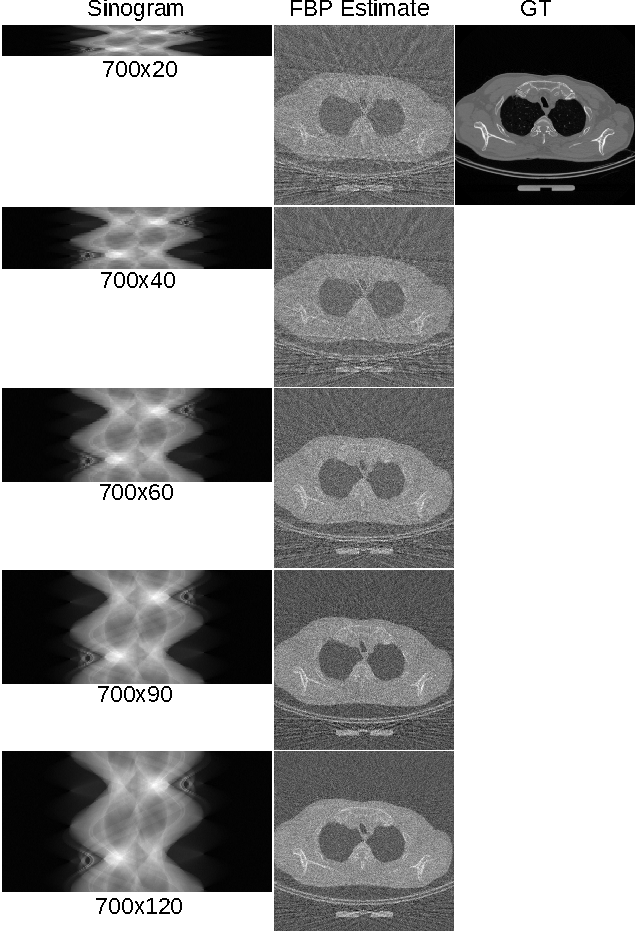
\includegraphics[width=0.75\linewidth]{dataset-crop.pdf}
	\caption{Samples from the dataset: Sinograms with different sparse-view configurations along with their corresponding \ac{FBP} estimate.}
	\label{fig:data}
\end{figure}

\section{Training}

We implemented the architectures described in the previous section using TensorFlow and Keras \cite{abadi2016tensorflow,chollet2015keras}. A subset of the dataset consisting of 22,000 \ac{2D} \ac{CT} images was used in this study. We then split the data into 30,000 images for training and 2,000 images for testing. The sinograms and \ac{FBP} estimates were generated using the ASTRA toolbox as described above. The sinograms were resized to $512 \times 512$ to ensure symmetry with the images for easier training of the network. The \ac{FBP} estimates $\boldxhat_1$ and $\boldxhat_2$ were resized to the resolutions required for concatenation to the proposed networks. The neural networks were independently trained for each of the sparse-view settings with $N_\mathrm{a}=20,40,60,90$ and $120$. The choice of $\boldx_1$ and $\boldx_2$ were at $64\times64$ and $128\times128$ resolutions for \ac{LRRCED}(D) and $128\times128$ and $256\times256$ resolutions for \ac{LRRCED}(U). The networks were trained for $50$ epochs with Adam optimizer with a decay of $10^{-4}$.


\section{Quantitative Analysis:}

The metrics used for evaluating the reconstructed images were \ac{SSIM} and \ac{PSNR}. They are defined as follows:
\begin{equation}
\mathrm{SSIM}(\boldx^\star,\boldx) = \frac{(2\mu_{\boldx^\star}\mu_{\boldx}+c_{1})(2\sigma_{\boldx^\star\boldx}+c_{2})}{(\mu_{\boldx^\star}^2+\mu_{\boldx}^2+c_{1})(\sigma_{\boldx^\star}^2+\sigma_{\boldx}^2+c_{2})}   
\end{equation}
where $\mu_{\boldx^\star}$ and $\mu_{\boldx}$ are the mean of $\boldx^\star$ and $\boldx$ respectively, $\sigma_{\boldx^\star}^2$ and $\sigma_{\boldx}^2$ are the variance of $\boldx^\star$ and $\boldx$, $\sigma_{\boldx^\star\boldx}$ is the covariance between $\boldx^\star$ and $\boldx$ , $c_{1}=(k_{1}L)^2$ and $c_{2}=(k_{2}L)^2$ where $k_{1}=0.01$ and $k_{2}=0.03$ by default,
\begin{equation}
\mathrm{PSNR} = 20\log_{10}\left(\frac{L-1}{\mathrm{RMSE}}\right)
\end{equation}
where $L$ is the maximum intensity in the image and \ac{RMSE} is given by
\begin{equation}
%    \mathrm{RMSE}(Y_\mathrm{true},Y_\mathrm{predicted}) = \sqrt{\frac{1}{n}   \sum_{i=1}^{n} (Y_\mathrm{true}^i-Y_\mathrm{predicted}^i)^2} 
\mathrm{RMSE}(\boldx^\star,\boldxhat) = \sqrt{\frac{1}{m}   \sum_{j=1}^{m} (x^\star_j-\xhat_j )^2} \, .
\end{equation}



\section{Comparative Analysis}

The  \ac{LRRCED} method was compared with a post-processing deep learning-based approach, namely FBP-ConvNet \cite{jin2017deep}, and a \ac{PWLS}-\ac{TV} solver for the model-based iterative \ac{CT} reconstruction \cite{tang2009performance}. We trained FBP-ConvNet on a set of 30,000 noisy, artifact-ridden \ac{FBP} image and \ac{GT} pairs. This network was trained for 50 epochs. 

\section{Results} \label{sec:results}

\subsection{Experimental Results}

Fig.~\ref{fig:d_ang} shows the images reconstructed with \ac{LRRCED}(D) for various degrees of sparsity in the projections. Images from various parts of the patient volume are displayed at different HUT windows for clearer evaluation of the proposed approach. We observe the improvement in the reconstructed images with the decrease in sparsity in the views. The images reconstructed with $N_\mathrm{a}=120$ appear closest to the \ac{GT}. The soft tissue regions in the images reconstructed with <60 views show artifacts which are not present with the use of more projections. Similarly in Fig.~\ref{fig:u_ang}, we show the images reconstructed with \ac{LRRCED}(U).  

In Fig.~\ref{fig:res_60} and Fig.~\ref{fig:res_90} we present a comparison of reconstructed images using different algorithms with 60 and 90 views respectively. The top row consists of the \ac{GT} and the reconstructed image by proposed \ac{LRRCED}(D) approach. The second row consists of  images with \ac{LRRCED}(U) and the FBP-ConvNet. Finally in the last row are the images reconstructed with \ac{PWLS}-\ac{TV} iterative method and \ac{FBP}. The region highlighted in yellow is zoomed and displayed alongside the corresponding image. These methods are quantitatively compared in Table~\ref{table:2} and Table~\ref{table:3}. We observe that the deep learning methods perform better than the iterative and analytical methods. The images reconstructed with U-Net based methods namely LRRCED(U) and FBP-ConvNet, have very similar characteristics: The contrast is higher and they perform better quantitatively. However, images reconstructed with DenseNet by comparison show less noise and streaking artifacts. These visual observations can be more clearly seen in the zoomed images shown in Fig.~\ref{fig:res_60}. This is further reiterated in the intensity plot profiles shown in Fig.~\ref{fig:ip_60} and Fig.~\ref{fig:ip_90}, where the LRR-CED(D) results are closer to the GT. In accordance with the metrics tabulated in Table~\ref{table:2} and Table~\ref{table:3}, we find that the plots of deep learning-based methods are very close to that of the \ac{GT}. Even though the proposed approach with typical \acp{CED} performs a task which is more complex than denoising, the metrics indicate that the quality has not deteriorated compared to a standard post-processing approach. 


\begin{figure*}[!htbp]
	\centering
	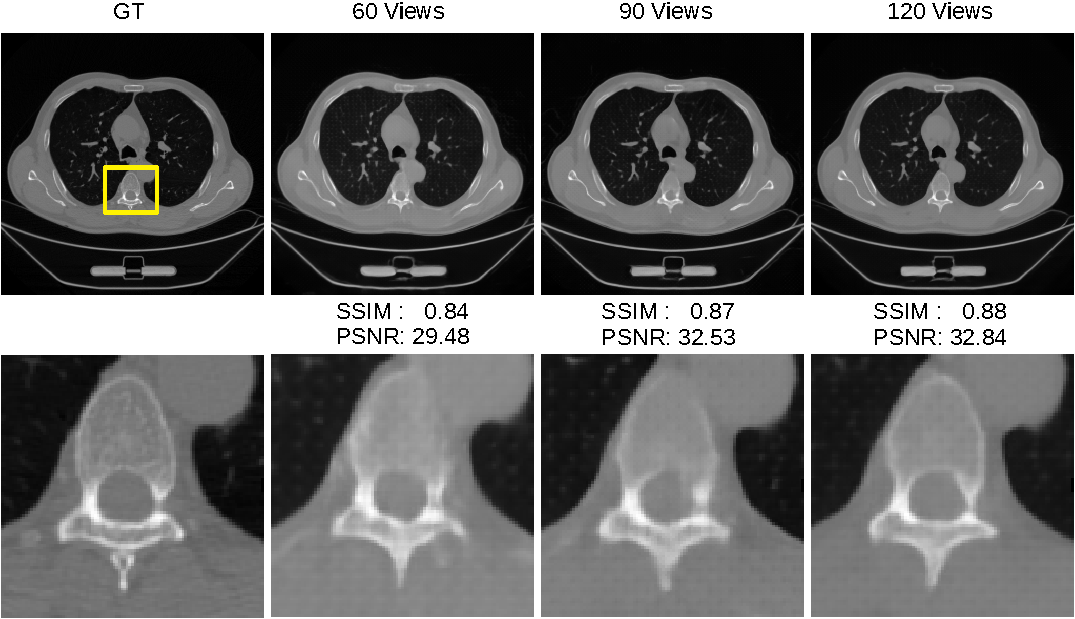
\includegraphics[width=1.00\linewidth]{views_dense-crop.pdf}
	\caption{Images reconstructed with LRR-CED(D) approach with different sparse-view configurations, i.e., projections with $N_\mathrm{a}=120,90,60,40$ and $20$. For better visual inspection images in first row are displayed in $-40 \pm 600$ HUT window, the second row in $-340 \pm 400$ HUT and the third in $-150 \pm 400$ HUT.}
	\label{fig:d_ang}
\end{figure*}


\begin{figure*}[!htbp]
	\centering
	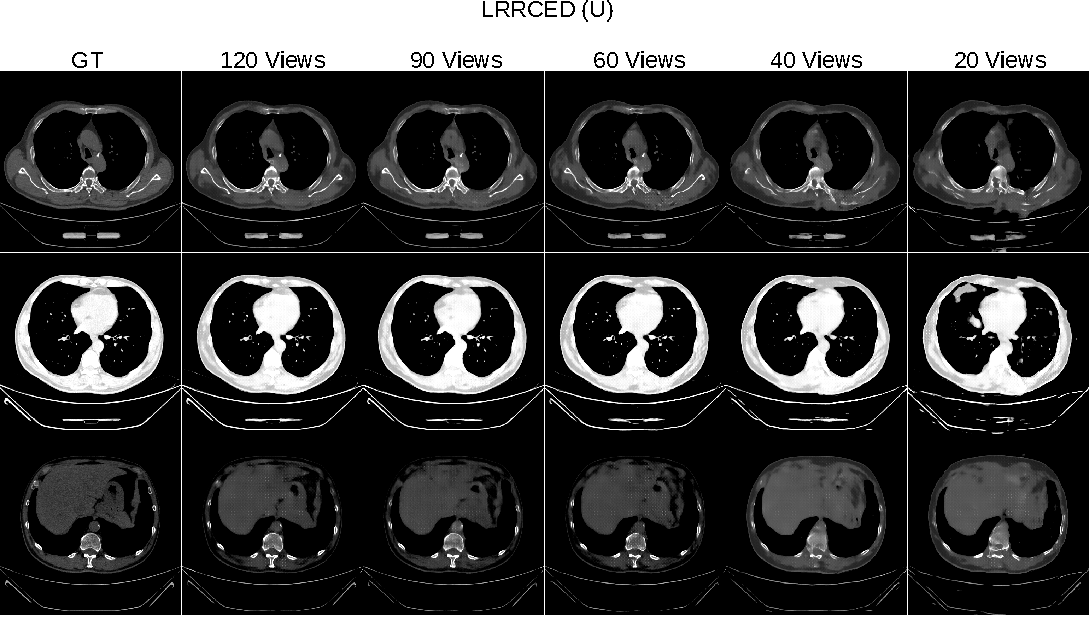
\includegraphics[width=1.00\linewidth]{views-unet-crop.pdf}
	\caption{Images reconstructed with LRR-CED(U) approach with different Sparse-View configurations, i.e., projections with $N_\mathrm{a}=120,90,60,40$ and $20$. Images in first row are displayed in $-40 \pm 600$ HUT window, the second row in $-340 \pm 400$ HUT and the third in $-150 \pm 400$ HUT.}
	\label{fig:u_ang}
\end{figure*}


\begin{table}[ht!]
	\centering
	\caption{Quantitative comparison of various reconstruction algorithms with \ac{SSIM} and \ac{PSNR} for projections with 60 views}
	\label{table:2}
	\begin{tabular}{||c|c|c|c|c|c||} 
		\hline
		Metric & FBP & PWLS-TV & FBP & \ac{LRRCED} & \ac{LRRCED}  \\ %[0.5ex] 
		&     &         & ConvNet & (D) & (U) \\
		\hline\hline
		SSIM & $0.16$ & $0.66$ & $0.90$ & $0.89$ & $0.90$ \\ 
		PSNR & $11.57$ & $28.23$ & $31.58$ & $30.04$ & $30.20$ \\   
		\hline  
		
		\hline  
	\end{tabular}
	
\end{table}

\begin{table}[ht!]
	\centering
	\caption{Quantitative comparison of various reconstruction algorithms with \ac{SSIM} and \ac{PSNR} for projections with 90 views}
	\label{table:3}
	\begin{tabular}{||c|c|c|c|c|c||} 
		\hline
		Metric & FBP & PWLS-TV & FBP & \ac{LRRCED} & \ac{LRRCED}  \\ %[0.5ex] 
		&     &         & ConvNet & (D) & (U) \\
		\hline\hline
		SSIM & $0.19$ & $0.72$ & $0.93$ & $0.91$ & $0.92$ \\ 
		PSNR & $13.57$ & $30.21$ & $35.27$ & $32.70$ & $32.86$ \\   
		\hline  
		
		\hline  
	\end{tabular}
	
\end{table}

\begin{figure}[!t]
	\centering
	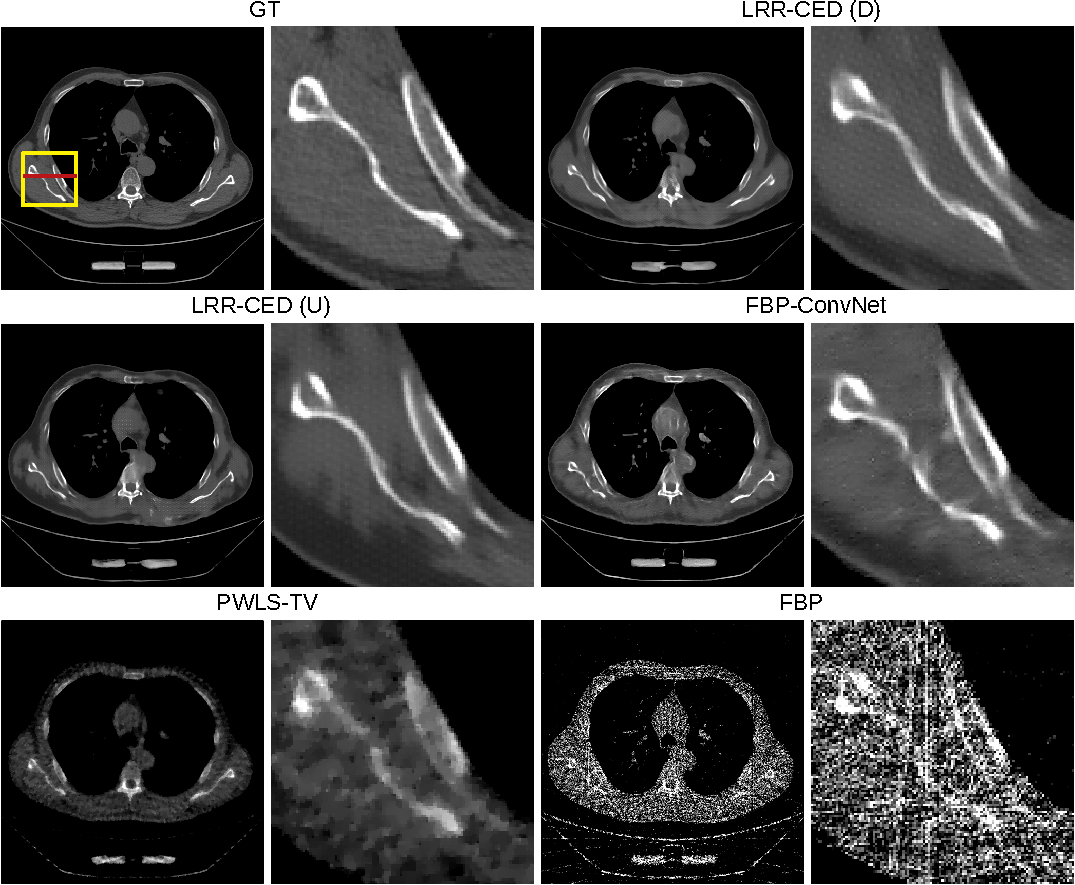
\includegraphics[width=0.9\linewidth]{60_views-crop.pdf}
	\caption{Comparative analysis for 60 views: From the top left corner, we have \ac{GT} image, reconstructions with \ac{LRRCED}(D) . In the second row reconstructed images with \ac{LRRCED}(U) and FBP-ConvNet. Finally images reconstructed with PWLS-TV and \ac{FBP}.}
	\label{fig:res_60}
\end{figure}




\begin{figure}[!t]
	\centering
	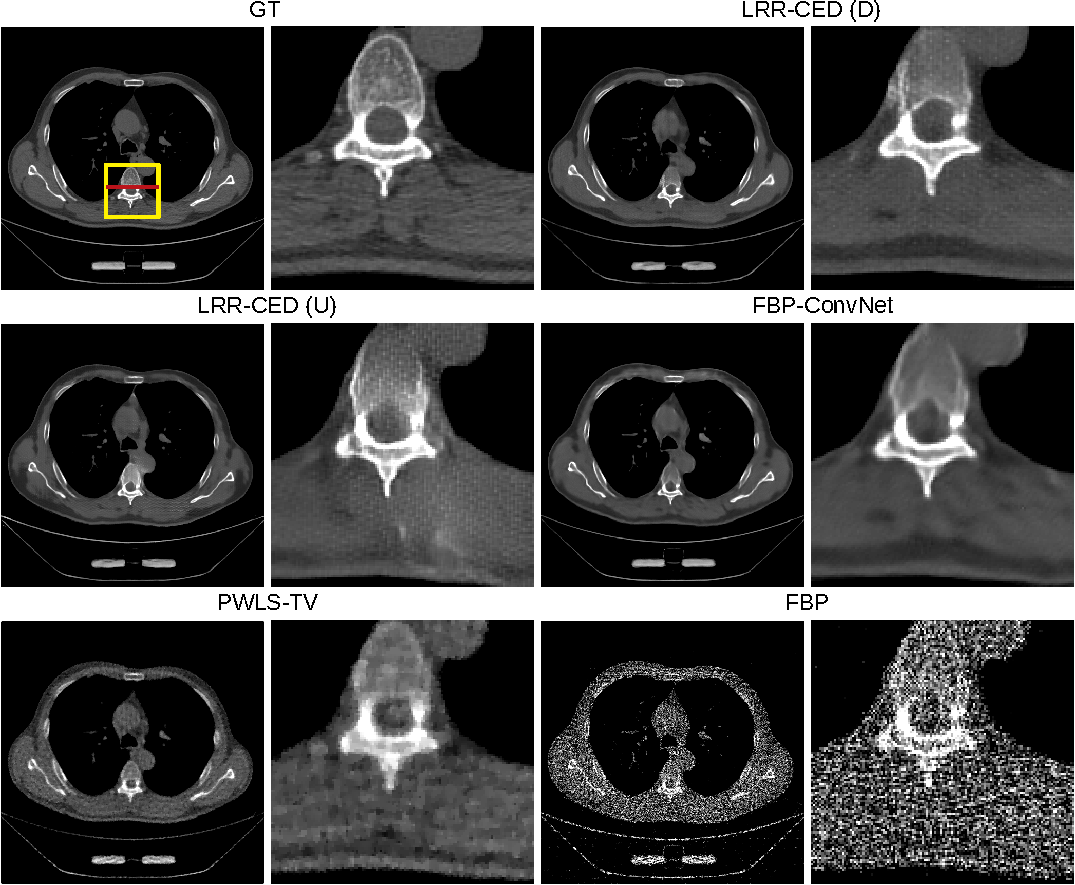
\includegraphics[width=0.9\linewidth]{90_views-crop.pdf}
	\caption{Comparative analysis for 90 views: From the top left corner, we have \ac{GT} image, reconstructions with \ac{LRRCED}(D) . In the second row reconstructed images with \ac{LRRCED}(U) and FBP-ConvNet. Finally images reconstructed with PWLS-TV and \ac{FBP}.}
	\label{fig:res_90}
\end{figure}


\begin{figure}
	\begin{subfigure}{.5\textwidth}
		\centering
		\begin{tikzpicture}[scale=0.9] 
		\begin{axis}[
		% title=X-ray source Energy: $140$ keV,
		mark options={mark size = 3pt},
		xlabel={Distance (in pixels)},
		ylabel={Attenuation (mm$^{-1}$)},
		xmin = 16,
		xmax = 116,
		grid = major,
		legend columns=2,
		legend cell align=left,
		legend entries={\ac{GT},\ac{LRRCED}(D),FBP-ConvNet},
		legend style={at={(0.5,1.2)},anchor=north}
		]
		\addplot[color=green, style={thick}] table[x=Distance, y=GT] {./Figures/60_views.txt};
		\addplot[color=red, style={thick}] table[x=Distance, y=LRR-CED(D)] {./Figures/60_views.txt};
		\addplot[color=black, style={thick}] table[x=Distance, y=FBP-ConvNet] {./Figures/60_views.txt};
		\end{axis}
		\end{tikzpicture}
		\caption{60 views 1}
		\label{fig:ip_60_d}
	\end{subfigure}%
	\begin{subfigure}{.5\textwidth}
		\centering
		\begin{tikzpicture}[scale=0.9] 
		\begin{axis}[
		mark options={mark size = 3pt},
		xlabel={Distance (in pixels)},
		ylabel={Attenuation (mm$^{-1}$)},
		xmin = 16,
		xmax = 116,
		grid = major,
		legend columns=2,
		legend cell align=left,
		legend entries={\ac{GT},\ac{LRRCED}(U),FBP-ConvNet},
		legend style={at={(0.5,1.2)},anchor=north}
		]
		\addplot[color=green, style={thick}] table[x=Distance, y=GT] {./Figures/60_views.txt};
		\addplot[color=blue, style={thick}] table[x=Distance, y=LRR-CED(U)] {./Figures/60_views.txt};
		\addplot[color=black, style={thick}] table[x=Distance, y=FBP-ConvNet] {./Figures/60_views.txt};
		\end{axis}
		\end{tikzpicture}
		\caption{60 views 2}
		\label{fig:ip_60_u}
	\end{subfigure}%
	\caption{Intensity plot profile for the region marked in red from Fig.~\ref{fig:res_60} comparing \ac{LRRCED}(D) and FBP-ConvNet to the \ac{GT} in \subref{fig:ip_60_d} and \ac{LRRCED}(U) and FBP-ConvNet in \subref{fig:ip_60_u}}
	\label{fig:ip_60}
\end{figure}

\begin{figure}
	\begin{subfigure}{.5\textwidth}
		\centering
		\begin{tikzpicture}[scale=0.9] 
		\begin{axis}[
		mark options={mark size = 3pt},
		xlabel={Distance (in pixels)},
		ylabel={Attenuation (mm$^{-1}$)},
		xmin = 200,
		xmax = 300,
		grid = major,
		legend columns=2,
		legend cell align=left,
		legend entries={\ac{GT},\ac{LRRCED}(D),FBP-ConvNet},
		legend style={at={(0.5,1.2)},anchor=north}
		]
		\addplot[color=green, style={thick}] table[x=Distance, y=GT] {./Figures/90_views.txt};
		\addplot[color=red, style={thick}] table[x=Distance, y=LRR-CED(D)] {./Figures/90_views.txt};
		\addplot[color=black, style={thick}] table[x=Distance, y=FBP-ConvNet] {./Figures/90_views.txt};
		\end{axis}
		\end{tikzpicture}
		\caption{90 views 1}
		\label{fig:ip_90_d}
	\end{subfigure}%
	\begin{subfigure}{.5\textwidth}
		\centering
		\begin{tikzpicture}[scale=0.9] 
		\begin{axis}[
		mark options={mark size = 3pt},
		xlabel={Distance (in pixels)},
		ylabel={Attenuation (mm$^{-1}$)},
		xmin = 200,
		xmax = 300,
		grid = major,
		legend columns=2,
		legend cell align=left,
		legend entries={\ac{GT},\ac{LRRCED}(U),FBP-ConvNet},
		legend style={at={(0.5,1.2)},anchor=north}
		]
		\addplot[color=green, style={thick}] table[x=Distance, y=GT] {./Figures/90_views.txt};
		\addplot[color=blue, style={thick}] table[x=Distance, y=LRR-CED(U)] {./Figures/90_views.txt};
		\addplot[color=black, style={thick}] table[x=Distance, y=FBP-ConvNet] {./Figures/90_views.txt};
		\end{axis}
		\end{tikzpicture}
		\caption{90 views 2}
		\label{fig:ip_90_u}
	\end{subfigure}%
	\caption{Intensity plot profile for the region marked in red from Fig.~\ref{fig:res_90} comparing \ac{LRRCED}(D) and FBP-ConvNet to the \ac{GT} in \subref{fig:ip_90_d} and \ac{LRRCED}(U) and FBP-ConvNet in \subref{fig:ip_90_u}}
	\label{fig:ip_90}
\end{figure}

\subsection{Experiments with real data}

The proposed networks were initialized with the weights from the previous study and were then trained on the real data. The real data used in this study was part of the Low Dose \ac{CT} grand challenge \cite{mccollough2016tu}. The data constituted of 10 patients, acquired with flying spot technique and a helical scan. It was a subset of the larger Mayo \ac{CT} clinic database \cite{moen2021low}. The data from nine patients constituting of 3,994 \ac{2D} slices was used for training and the trained network was tested on another patient data.  The \ac{3D} sinograms obtained from the helical scan were converted into \ac{2D} sinograms through the single slice re-binning method employed in \cite{kim2017low}. We further resampled the sinograms reducing the number of views to 64. The number of detector panels was 734. The \ac{FBP} estimates were generated from these sparse-view sinograms and resized for training the \ac{LRRCED}.

We present the results for four different slices across the patient volume and their quantitative evaluation in Figure~\ref{fig:m1} and Table~\ref{table:m1}, respectively. We observe that the reconstructed images with the proposed networks have similar characteristics as the ones from the simulation study. The transfer learning strategy ensures that the quality of the reconstructed images is maintained even with very limited training data.



\begin{figure}[!t]
	\centering
	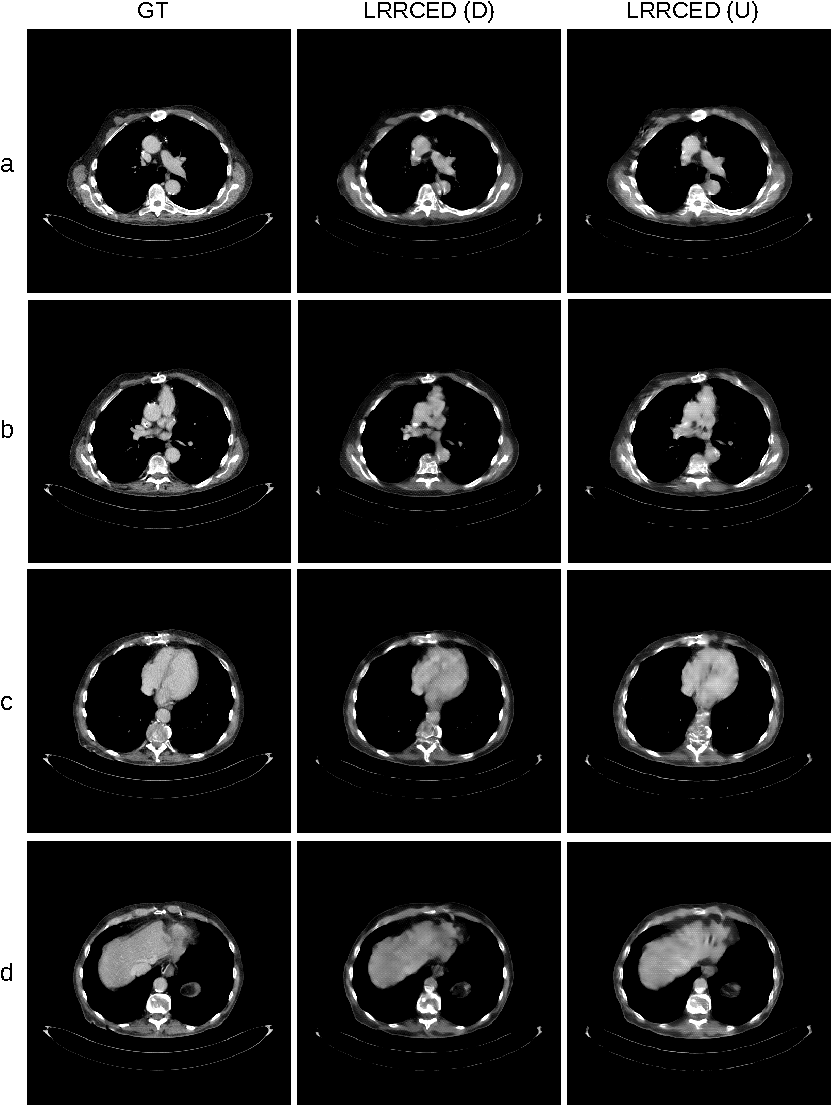
\includegraphics[width=0.8\linewidth]{./mayo-crop.pdf}\hfill
	\caption{Real data study: Images reconstructed with the proposed approaches across 4 different slices displayed in the window $40 \pm 200 $ HUT. }\label{fig:m1}
\end{figure}


\begin{table}[ht!]
	\centering
	\caption{Quantitative comparison of images reconstructed with the proposed algorithms w.r.t. \ac{GT} across different slices in the patient volume from the real dataset displayed in Fig.~\ref{fig:m1}}
	\label{table:m1}
	\begin{tabular}{||c|c|c|c||} 
		\hline
		Image & Metric  & LRRCED(D) & LRRCED(U) \\ %[0.5ex] 
		\hline\hline
		a & SSIM      & $0.89$ & $0.92$ \\ 
		&  PSNR      & $35.70$ & $36.64$  \\   
		\hline  
		b & SSIM      & $0.88$ & $0.92$ \\ 
		& PSNR      & $35.19$ & $36.13$  \\   
		\hline
		c & SSIM      & $0.94$ & $0.92$ \\ 
		& PSNR      & $40.86$ & $42.04$  \\   
		\hline
		d & SSIM      & $0.84$ & $0.91$ \\ 
		& PSNR      & $33.37$ & $34.59$  \\   
		\hline
		
	\end{tabular}
	
\end{table}

\subsection{Stability Study}
One of the major challenges to data-driven neural network approaches is the ability to generalize over different types of test data. The extent to which a neural network is stable when presented with data different from the training data is the focus of this study. This topic has been extensively evaluated in the article by \cite{antun2020instabilities}. The authors analyzed the impact of tiny perturbations and small structural changes in sampling and image domain on the reconstructed images. They also observed the way in which a change in sampling (sparsity in \ac{CT} for example) could influence performance. In our work centered around sparse-view \ac{CT} image reconstruction, we performed a series of experiments with different levels of sparsity in the testing data. The proposed network \ac{LRRCED}(D) was trained separately on each of the sparsity configurations, ($N_\mathrm{a}= 20,40,60,90 \: \mathrm{and} \:  120$). It was then tested using the sinograms and the corresponding \ac{FBP} estimates for all of the possible values of $N_\mathrm{a}$ considered.

The results are displayed in Fig~\ref{fig:ins1}. The top row corresponds to network trained with 20-view data, the second with 40-view data and so on. The trend is towards an improvement in overall image quality with reduced sparsity in the sinograms. On one hand, we observe that in the scenarios where the testing data has more sparsity than the training data, the artifacts in the reconstructed images are more clearly visible. This is clearly seen in the last two rows in Figure~\ref{fig:ins1}, where the network was trained on 90 views and 120 views data and the images  reconstructed with lower $N_\mathrm{a}$ are ridden with artifacts. On the other hand, the image quality especially in the soft tissue regions is higher when the network is trained and tested on data with more views. The proposed network maintains stability in the reconstructed images with the increase in the sampling in the testing data. However, when the testing data has fewer views than the training data, artifacts are present in the reconstructed images.
\begin{figure}[!t]
	\centering
	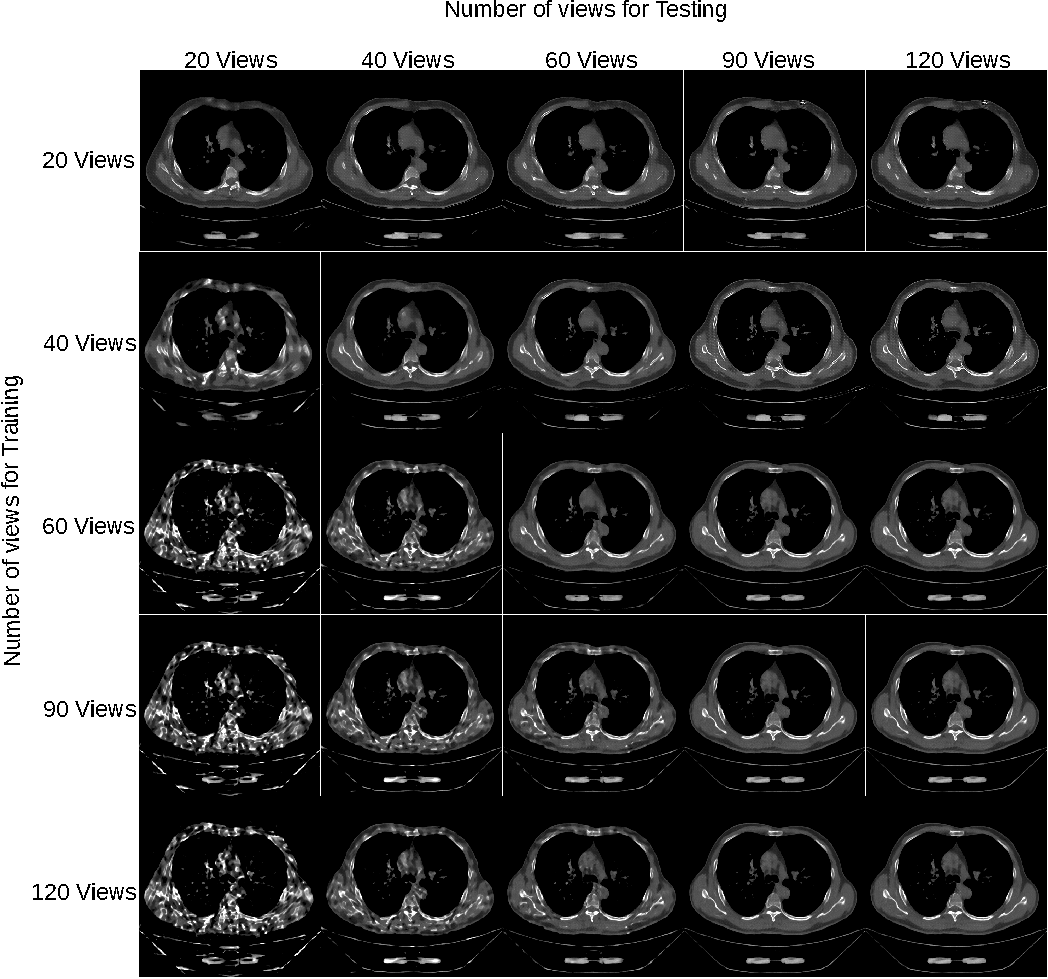
\includegraphics[width=1.0\linewidth]{./instab_1-crop.pdf}\hfill
	\caption{Stability study: Each row corresponds to the network trained on specific value of $N_\mathrm{a}$, and tested with all the possible values of $N_\mathrm{a}$.}\label{fig:ins1}
\end{figure}

\subsection{Hyperparameter optimization}

Finding the optimal hyperparameters is an important aspect of training neural networks. The common hyperparameters in a typical \ac{CNN} are number of filters, number of layers, etc. These interdependent hyperparameters  determine the rate of convergence and require task-specific experimentation to arrive at the best possible configuration. The unique hyperparameters in our proposed approach are the resolutions of concatenated \ac{FBP} estimates. The number of training examples is another important component that varies depending on the task and the trainable parameters of the neural network selected for the task. In this section we discuss our experiments that determined the selection of these two important hyperparameters. 

\subsubsection{Concatenation Resolution Selection} \label{sec:concat}

To select the best possible configuration for concatenation in the proposed approach, we trained the networks with a fixed set of hyper-parameters and different combinations of concatenations. We discuss the results with \ac{LRRCED}(D) in this regard. The number of training samples were set to 10,000 for all the experiments. The training data were projections with 90 views, corresponding \ac{FBP} reconstructed images and the \ac{GT}. The training was done for 25 epochs. Each of the concatenation setting was evaluated on 5 test patients. The average \ac{SSIM} for each patient was plotted for each of the experiment setting. In Fig~\ref{fig:c1} we have the average \ac{SSIM} vs Patient plot for single concatenation at a specific resolution. Similarly Figure~\ref{fig:c2} consists of plots for double concatenation at two different resolutions. The double concatenation at $64\times64, 128\times128$ overall leads to the best metrics, thus becoming our choice for the experiments in this work. These results are tabulated in Table~\ref{table:5}.



\subsubsection{Training Examples Analysis}

One of the biggest challenges in any data driven algorithm is the selection of training examples required for the experiments. It is important to analyze this hyper-parameter as it serves as an important factor for the network to be reproducible and scalable. We varied the number of training examples for the best concatenation setting from the previous section and the 90-view scenario. The evaluation was similar to the previous experiment with the average \ac{SSIM} for 5 patients. The results from these experiments are tabulated in Table~\ref{table:6}. As seen in Figure~\ref{fig:tr}, the performance of the network improves along with the increase in the number of training examples. There is however a marginal difference in the performance of the network when trained with 20,000 or 30,000 training examples, hence making us choose 20,000 training examples as the optimum number for this hyper-parameter. The average \ac{SSIM} values across the test patients tend to get similar as the number of training examples increases.

\subsection{Ablation Study} \label{sec:ablation}

We performed an ablation study to understand the impact of the proposed concatenations on the neural network performance. DenseNet described earlier was trained for 50 epochs on 20,000 data samples in three different scenariosas shown in Figure~\ref{fig:a2}, two of which used either a sinogram consisting of randomly distributed Gaussian noise and no low-resolution concatenations: (i) true sinogram and the reconstructed image only (no low-resolution concatenations), (ii) Gaussian noise sinogram, low-resolution concatenations and the reconstructed images, and (iii) true sinogram, low-resolution concatenations and the reconstructed images. 

The image predictions by the three different neural networks are shown in Figure~\ref{fig:a1}. DenseNet without the low-resolution concatenations does produce images with some structural information, but the other two configurations generate images of much better quality. We observe that the concatenations indeed help the network learn the structure of the image, while the sinograms contribute in artifact and noise removal. This is reflected upon closer inspection of the third and fourth images in Figure~\ref{fig:a1}. The images predicted with \ac{LRRCED}(D) trained using the randomly distributed Gaussian noise sinogram instead of the true sinogram have artifacts and noise which is also seen quantitatively in Table~\ref{table:7}. The best metrics and image quality are demonstrated by the neural network trained on the combination of sinograms and low-resolution estimates labeled as \ac{LRRCED}(D) in Figure~\ref{fig:a1}. 



\begin{table}[ht!]
	\centering
	\caption{Average \ac{SSIM} for different configurations of concatenations}
	\label{table:5}
	\begin{tabular}{||c|c|c|c|c|c||} 
		\hline
		Concatenated & \multicolumn{5}{c||}{Average \ac{SSIM}}  \\ \cline{2-6}%[0.5ex] 
		\ac{FBP} Resolution &   P1  &  P2     & P3 & P4 & P5 \\
		\hline\hline
		$(32\times32)$ & $0.82$ & $0.86$ & $0.88$ & $0.86$ & $0.80$ \\ 
		$(64\times64)$ & $0.85$ & $0.88$ & $0.90$ & $0.88$ & $0.82$ \\   
		$(128\times128)$ & $0.85$ & $0.87$ & $0.90$ & $0.89$ & $0.81$ \\   
		$(256\times256)$ & $0.58$ & $0.88$ & $0.85$ & $0.88$ & $0.79$ \\   
		$(512\times512)$ & $0.66$ & $0.78$ & $0.82$ & $0.75$ & $0.73$ \\   
		\hline
		$(32\times32,64\times64)$ & $0.83$ & $0.77$ & $0.80$ & $0.80$ & $0.68$ \\   
		$\mathbf{(64\times64,128\times128)}$ & $\mathbf{0.85}$ & $\mathbf{0.88}$ & $\mathbf{0.91}$ & $\mathbf{0.89}$ & $\mathbf{0.83}$ \\   
		$(128\times128,256\times256)$ & $0.67$ & $0.78$ & $0.83$ & $0.84$ & $0.70$ \\   
		\hline  
		
		\hline  
	\end{tabular}
	
\end{table}

\begin{table}[ht!]
	\centering
	\caption{Average \ac{SSIM} for different number of training examples}
	\label{table:6}
	\begin{tabular}{||c|c|c|c|c|c||} 
		\hline
		Number of Training  & \multicolumn{5}{c||}{Average \ac{SSIM}}  \\ \cline{2-6}%[0.5ex] 
		examples &   P1  &  P2     & P3 & P4 & P5 \\
		\hline\hline
		$1,000$ & $0.82$ & $0.79$ & $0.86$ & $0.85$ & $0.72$ \\ 
		$5,000$ & $0.84$ & $0.77$ & $0.86$ & $0.84$ & $0.69$ \\   
		$10,000$ & $0.85$ & $0.88$ & $0.91$ & $0.89$ & $0.83$ \\   
		$\mathbf{20,000}$ & $\mathbf{0.89}$ & $\mathbf{0.90}$ & $\mathbf{0.91}$ & $\mathbf{0.90}$ & $\mathbf{0.82}$ \\   
		$30,000$ & $0.89$ & $0.89$ & $0.90$ & $0.90$ & $0.82$ \\   
		\hline  
		
		\hline  
	\end{tabular}
	\vspace{.5cm}
\end{table}



\begin{figure}[!h]
	\centering
	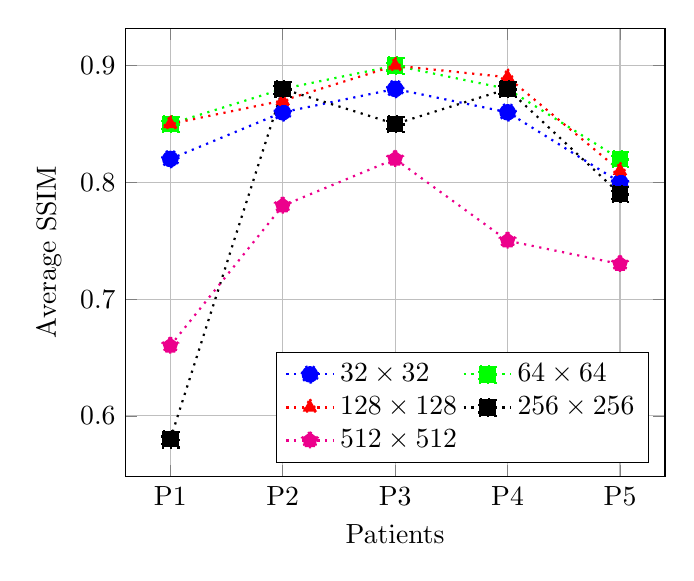
\begin{tikzpicture}[scale=1] 
	\begin{axis}[
	% title=X-ray source Energy: $140$ keV,
	mark options={mark size = 3pt},
	xlabel={Patients},
	ylabel={Average SSIM},
	xticklabels={,P1,P2,P3,P4,P5},
	grid = major,
	legend columns=2,
	legend cell align=left,
	legend entries={$32\times 32$,$64\times 64$,$128\times 128$,$256\times 256$,$512\times 512$},
	% legend entries={MCAOL,CAOL, Huber, TV, },
	legend style={legend pos=south east}
	]
	
	\addplot[color=blue, mark=*, style={thick,dotted}] coordinates   {(0,0.82)(10,0.86)(20,0.88)(30,0.86)(40,0.8)};
	\addplot[color=green, mark=square*, style={thick,dotted}] coordinates  {(0,0.85)(10,0.88)(20,0.9)(30,0.88)(40,0.82)};
	\addplot[color=red, mark=triangle*, style={thick,dotted}] coordinates  {(0,0.85)(10,0.87)(20,0.9)(30,0.89)(40,0.81)};
	\addplot[color=black, mark=square*, style={thick,dotted}] coordinates    {(0,0.58)(10,0.88)(20,0.85)(30,0.88)(40,0.79)};
	\addplot[color=magenta, mark=pentagon*, style={thick,dotted}] coordinates {(0,0.66)(10,0.78)(20,0.82)(30,0.75)(40,0.73)};
	
	\end{axis}
	\end{tikzpicture}
	
	\caption{Comparison of single concatenations for the particular case of 90 views evaluated with \ac{SSIM} on 5 different patients from the dataset. The best metrics are found with concatenation at $128\times 128$.}\label{fig:c1}
\end{figure}



\begin{figure}[!htbp]
	\centering
	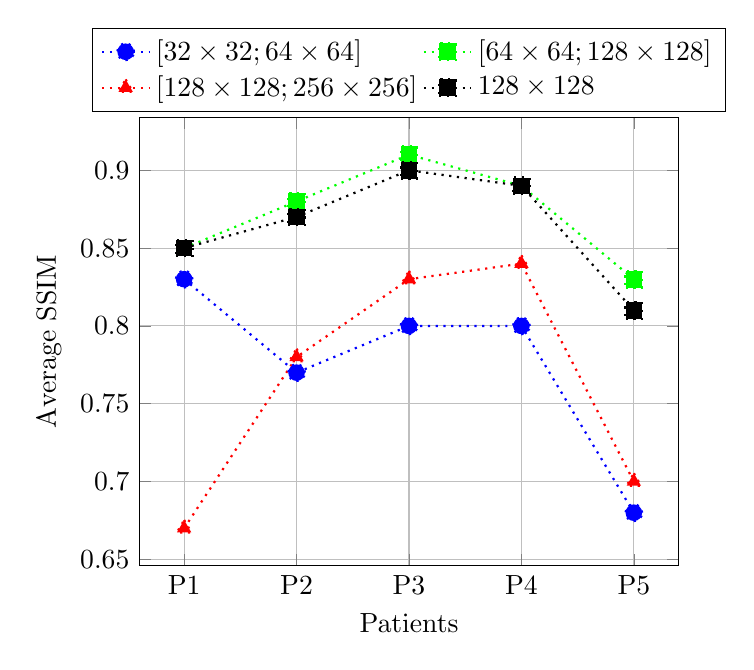
\begin{tikzpicture}[scale=1] 
	\begin{axis}[
	% title=X-ray source Energy: $140$ keV,
	mark options={mark size = 3pt},
	xlabel={Patients},
	ylabel={Average SSIM},
	xticklabels={,P1,P2,P3,P4,P5},
	grid = major,
	legend columns=2,
	legend cell align=left,
	legend entries={$[32\times 32 ; 64\times 64]$,$[64\times 64 ; 128\times 128]$,$[128\times 128 ; 256\times 256]$,$128\times 128$},
	% legend entries={MCAOL,CAOL, Huber, TV, },
	legend style={at={(0.5,1.2)},anchor=north}
	]
	
	\addplot[color=blue, mark=*, style={thick,dotted}] coordinates   {(0,0.83)(10,0.77)(20,0.8)(30,0.8)(40,0.68)};
	\addplot[color=green, mark=square*, style={thick,dotted}] coordinates  {(0,0.85)(10,0.88)(20,0.91)(30,0.89)(40,0.83)};
	\addplot[color=red, mark=triangle*, style={thick,dotted}] coordinates  {(0,0.67)(10,0.78)(20,0.83)(30,0.84)(40,0.7)};
	\addplot[color=black, mark=square*, style={thick,dotted}] coordinates    {(0,0.85)(10,0.87)(20,0.9)(30,0.89)(40,0.81)};
	
	\end{axis}
	\end{tikzpicture}
	
	\caption{Comparison of double concatenations for the particular case of 90 views evaluated with \ac{SSIM} on 5 different patients from the dataset. The best metrics are found with concatenations at $64\times 64$ and $128\times 128$ resolutions.}\label{fig:c2}
\end{figure}


\begin{figure}[!h]
	\centering
	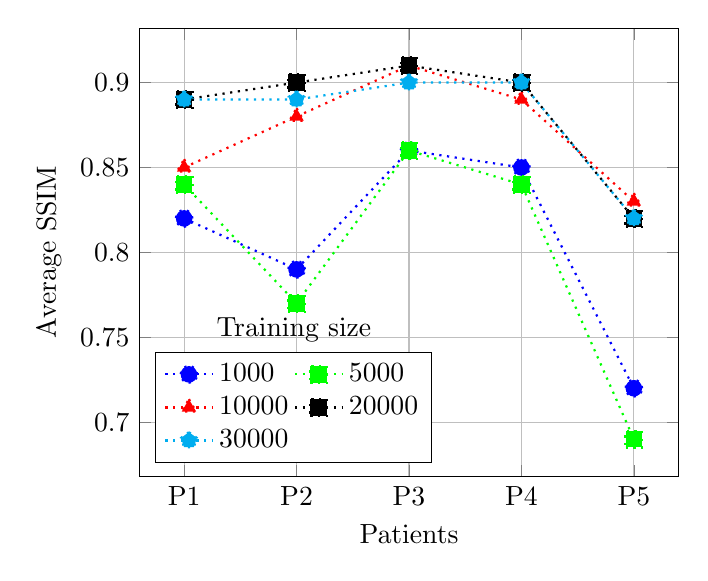
\begin{tikzpicture}[scale=1] 
	\begin{axis}[
	% title=X-ray source Energy: $140$ keV,
	mark options={mark size = 3pt},
	xlabel={Patients},
	ylabel={Average SSIM},
	xticklabels={,P1,P2,P3,P4,P5},
	grid = major,
	legend columns=2,
	legend cell align=left,
	legend entries={$1000$,$5000$,$10000$,$20000$,$30000$},
	% legend entries={MCAOL,CAOL, Huber, TV, },
	legend style={legend pos=south west,label=above:Training size}
	]
	
	\addplot[color=blue, mark=*, style={thick,dotted}] coordinates   {(0,0.82)(10,0.79)(20,0.86)(30,0.85)(40,0.72)};
	\addplot[color=green, mark=square*, style={thick,dotted}] coordinates  {(0,0.84)(10,0.77)(20,0.86)(30,0.84)(40,0.69)};
	\addplot[color=red, mark=triangle*, style={thick,dotted}] coordinates  {(0,0.85)(10,0.88)(20,0.91)(30,0.89)(40,0.83)};
	\addplot[color=black, mark=square*, style={thick,dotted}] coordinates    {(0,0.89)(10,0.9)(20,0.91)(30,0.9)(40,0.82)};
	\addplot[color=cyan, mark=pentagon*, style={thick,dotted}] coordinates {(0,0.89)(10,0.89)(20,0.9)(30,0.9)(40,0.82)};
	
	\end{axis}
	\end{tikzpicture}
	
	\caption{Comparison of Average \ac{SSIM} for 5 different Patient data for 90 views with varying number of training samples. The configuration of the network is the one with best performance from the analysis in Figure~\ref{fig:c1}. (concatenations at $64\times 64$ and $128\times 128$). }\label{fig:tr}
\end{figure}

\begin{figure}[!t]
\centering
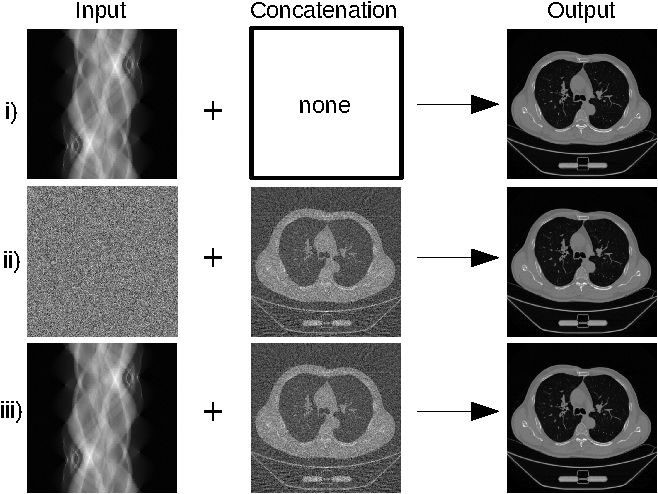
\includegraphics[width=0.5\linewidth]{./ab_rep-crop.pdf}\hfill
\caption{Schematic representation of configurations used in the ablation study: (i) true sinogram and the reconstructed image only (no low-resolution concatenations); (ii) randomly distributed Gaussian noise sinogram, low-resolution concatenations and the reconstructed images; (iii) true sinogram, low-resolution concatenations and the reconstructed images.}\label{fig:a2}
\end{figure}


\begin{figure}[!t]
\centering
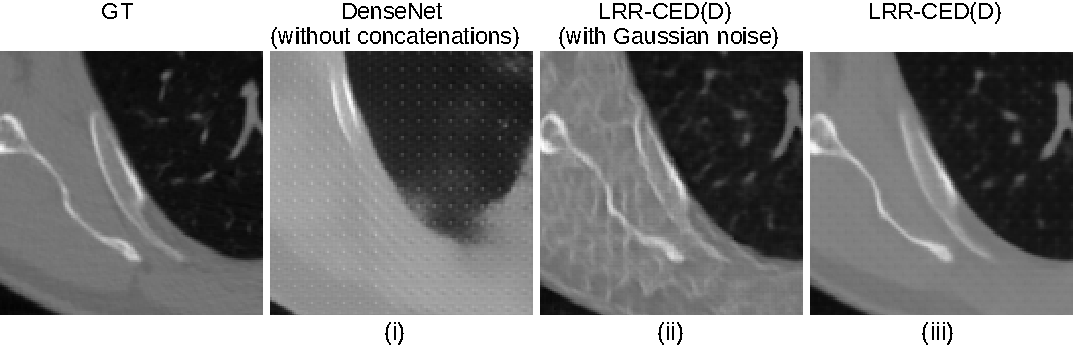
\includegraphics[width=1.0\linewidth]{./ablation-crop.pdf}\hfill
\caption{Ablation study: Predictions from different configurations of the network.\label{fig:a1}}
\end{figure}


\begin{table}[ht!]
\centering
\caption{Ablation Study: Quantitative comparison of different configurations of the DenseNet}
\label{table:7}
\begin{tabular}{||c|c|c|c|c|c||} 
	\hline
	Sl.No.    & True      & Concatenations   & Gaussian noise &    \ac{SSIM} &  \ac{PSNR}      \\ %[0.5ex] 
	& sinograms &                  &  sinograms     &              &                 \\
	\hline\hline
	(i)        &\cmark    &    \xmark       &    \xmark     &    $0.29$    &  $12.05$         \\     
	\hline
	(ii)       &\xmark    &    \cmark       &    \cmark     &    $0.70$    &  $28.89$         \\
	\hline  
	(iii)       &\cmark    &    \cmark       &    \xmark     &  $\bm{0.88}$ & $\bm{32.53}$     \\ 
	\hline
\end{tabular}

\end{table}


\section{Discussion} \label{sec:discussion}

The use of deep learning architectures in the framework of medical image reconstruction is propelled by potentially faster reconstruction without compromising on the quality of the images. To this end, hybrid image reconstruction involving unrolled iterative algorithms with embedded deep learning architectures do not significantly reduce the reconstruction time. Hence, the use of deep learning architectures for either improving images from a fast analytic algorithm or direct reconstruction becomes more relevant for their incorporation into the image reconstruction pipeline. One significant problem for direct image reconstruction is the requirement of large and complex networks to learn the mapping from sinograms to images without the help of any reconstruction estimate. The networks used for post-processing on the other hand are simpler and relatively easy to train. In this work we attempted to use these post-processing networks for the direct image reconstruction task along with low-resolution scout images from direct analytical method. We show that concatenating \ac{FBP} estimates at lower resolutions is sufficient to allow the network to learn the mapping from sinogram to image space. Through the use of two different networks with the concatenation approach we demonstrate that this idea can be applied to \acp{CED} in general.   

In the sparse-view \ac{CT} scenario artifact removal along with denoising increases the challenges of getting a clean well-resolved image. We observed that the use of traditional loss functions (L1 or L2) resulted in blurry images. To tackle this and to improve the sharpness of the images we used perceptual loss along with the standard L1 loss. The reconstructed images with our proposed \ac{LRRCED}(D) and \ac{LRRCED}(U) have higher \ac{SSIM} and \ac{PSNR} than images reconstructed with a traditional iterative algorithm and a standard post-processing deep learning method FBP-ConvNet. The similarity in the images from the deep learning methods stems from the fact that the choice of networks used in our proposed work was inspired from post-processing \acp{CED}. The contribution in this work is the use of these networks to learn the mapping from sparse sinograms to images with the same amount of training examples, which is possible only with the proposed addition of the concatenations. Through the ablation study from Section~\ref{sec:ablation}, we reiterate the contribution of both the sinogram and the low-resolution concatenations for image reconstruction. The \ac{CED} without the concatenations could learn the mapping but it would need much higher number of training examples for image quality comparable to other methods. The proposed method was compared to a U-Net based denoising method (FBP-ConvNet), which has one of the best quantitative metrics in image reconstruction as established by the recent quantitative comparison study carried out by \cite{leuschner2021quantitative}. As it was shown in this study, complex unrolled methods do only marginally better than the U-Net, hence making it one of the most frequently used benchmarks for comparison purposes. 

We are currently exploring the possibility of using image estimates from earlier iterations of standard iterative algorithms while ensuring that the trade-off between time and image quality is not compromised. The use of other alternative architectures is also being explored to arrive at reconstructed images which perform significantly better than existing post-processing approaches. Finally, we are working on experiments with low-dose \ac{CT} and other tomographic reconstruction modalities to establish the adaptability of the proposed approach.  

\section{Conclusion} \label{sec:conclusion}

In this work we studied the use of fully convolutional encoder-decoder networks in direct sparse-\ac{CT} image reconstruction. We introduced a new approach that uses lower dimension \ac{FBP} estimates as concatenations to help the network learn the mapping from sinogram to image space. In the context of image reconstruction, we inject the information from the inverse of a \ac{CT} physical system (\ac{FBP} estimate) as a feature map in the decoder. We presented two variations of the proposed approach namely \ac{LRRCED}(D) using fully convolutional dense networks and \ac{LRRCED}(U) using U-Net. The proposed neural networks reconstruct images that are either better or are on par with traditional reconstruction algorithms and post-processing deep learning based approach (FBP-ConvNet). A single pass of a sparse sinogram through the network results in reconstructed images without the artifacts and noise which are severely present in the concatenated \ac{FBP} estimates. Finally, this idea of using task specific concatenations that enable one to have control over what the network learns, can be extended to various other problems in medical imaging. 


